%\section{Threshold and color space Find which color space can isolate the iris the best}
\section[Threshold and color space Find which color space can isolate the iris the best]{Threshold and color space \\ Find which color space can isolate the iris the best}

\subsection{Method}
A good picture of the subject was taken, the quality of the image is highly dependant on the ligting as the contrast between the eyes and surrounding area needs to be high.

The approximate area surrounding the eyes was roughly cut out manually. The cropped image was put through the "Color Thresholder" app in matlab. The color spaces RGB, HSV, YCbCr \& L*a*b* were tried and only HSV \& YCbCr gave adequate results and was used to make two binary masks.


\begin{figure}[H]
    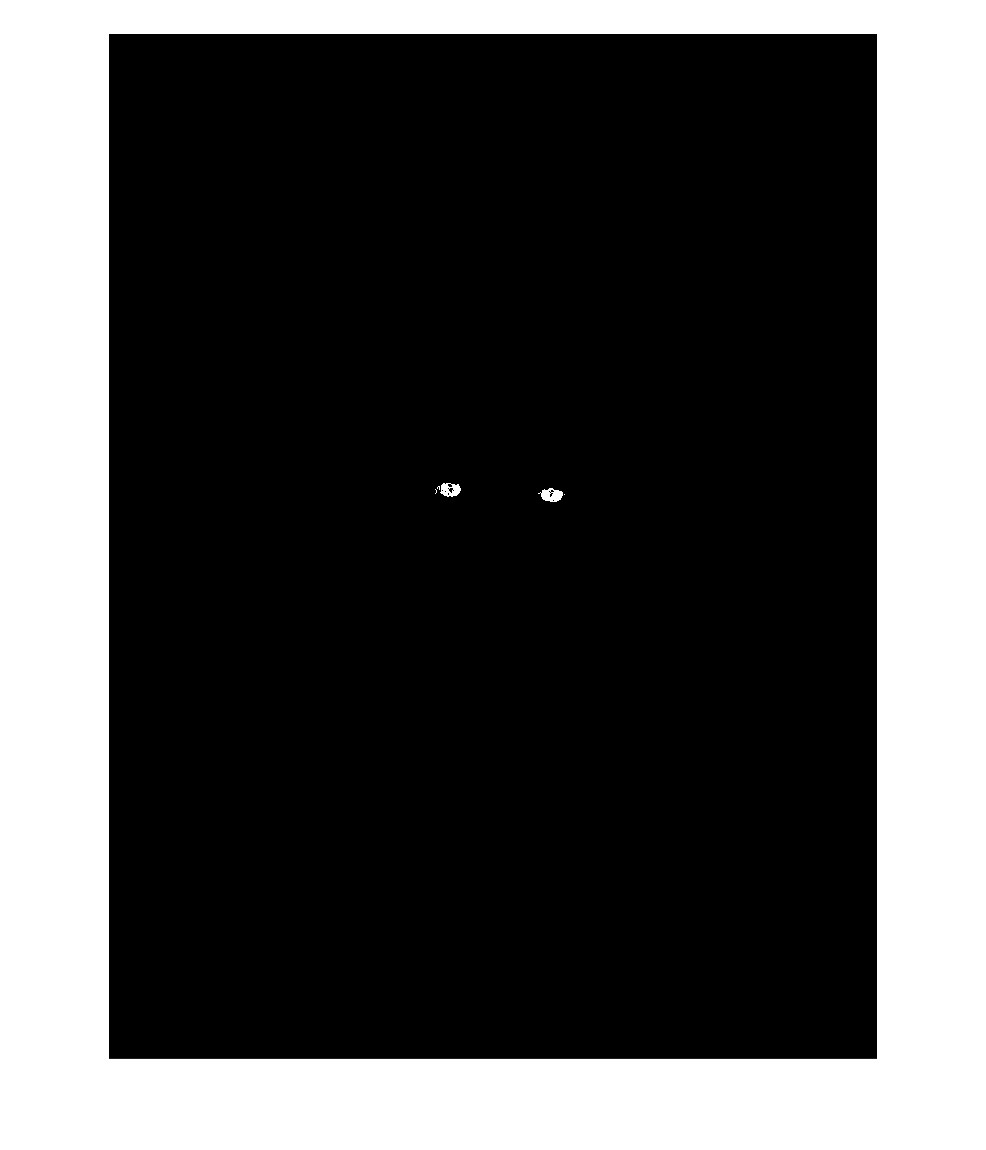
\includegraphics[width=0.3\textwidth]{./MaskofHSV.jpg}        
    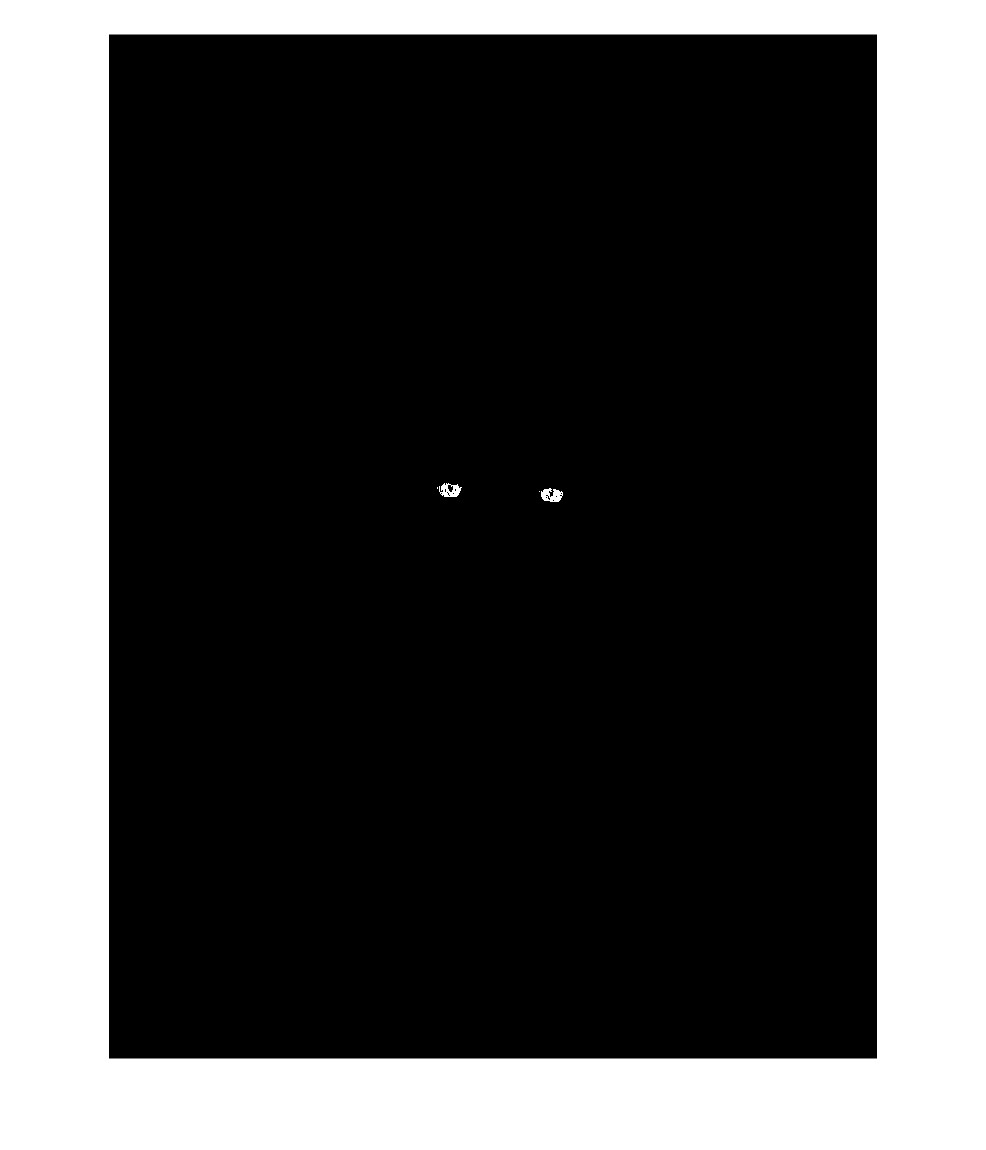
\includegraphics[width=0.3\textwidth]{./MaskofYbCbCr.jpg}
    \caption{Left image: The Mask created using the HSV color space. Right Image: The Mask created using the YbCbCr color space.}
    \label{fig:first}
\end{figure}

Using this mask an image with only eyes present and a image without eyes were created. The former had its RGB values shifted to make a predominantly red and a predominantly green version.

The two shifted imaged were then combined with the eyeless image to create a full image which only had a color shifted eyes.


\subsection{Result}
The resulting images of the HSV color space:
\begin{figure}[H]
    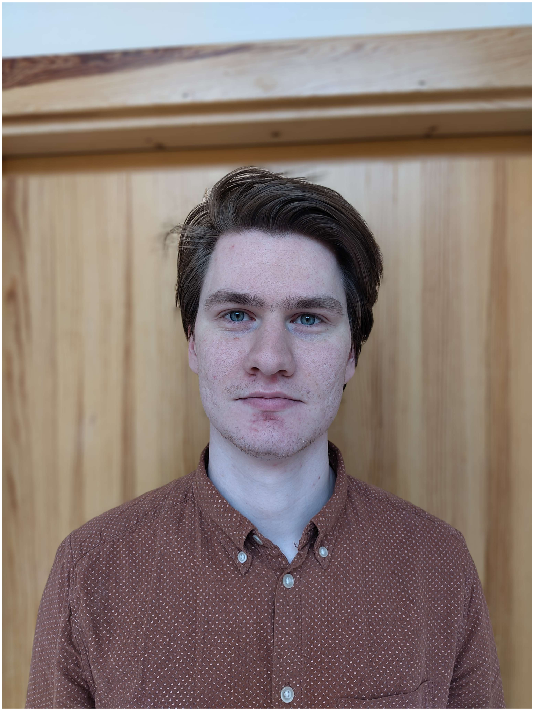
\includegraphics[width=0.3\textwidth]{./HSV_B.png}
    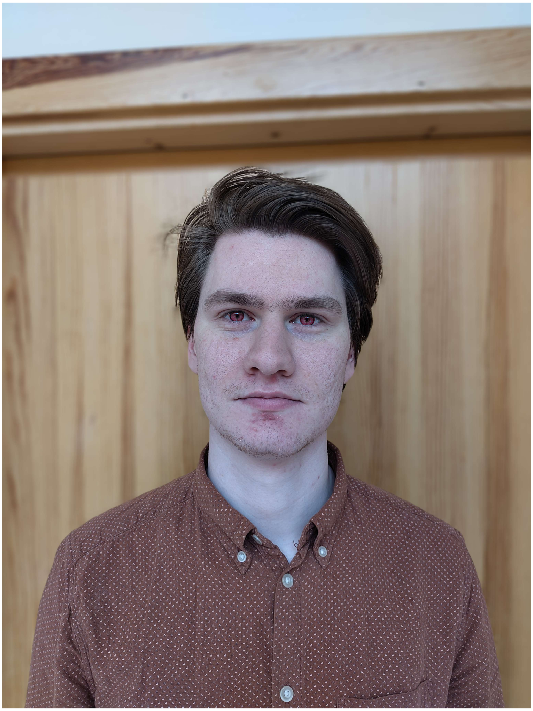
\includegraphics[width=0.3\textwidth]{./HSV_R.png}
    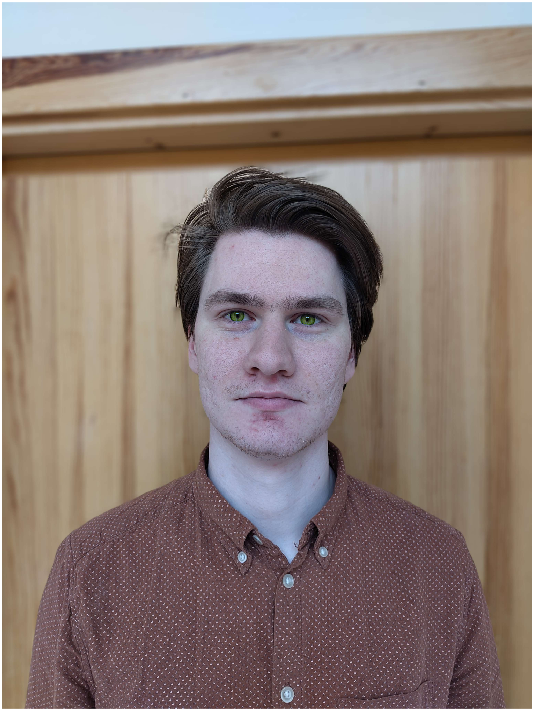
\includegraphics[width=0.3\textwidth]{./HSV_G.png}
    \caption{Left image: The Original image. Middle Image: The red shifted image. Right Image: The green shifted image.}
\end{figure}

The resulting images of the YbCbCr color space:
\begin{figure}[H]
    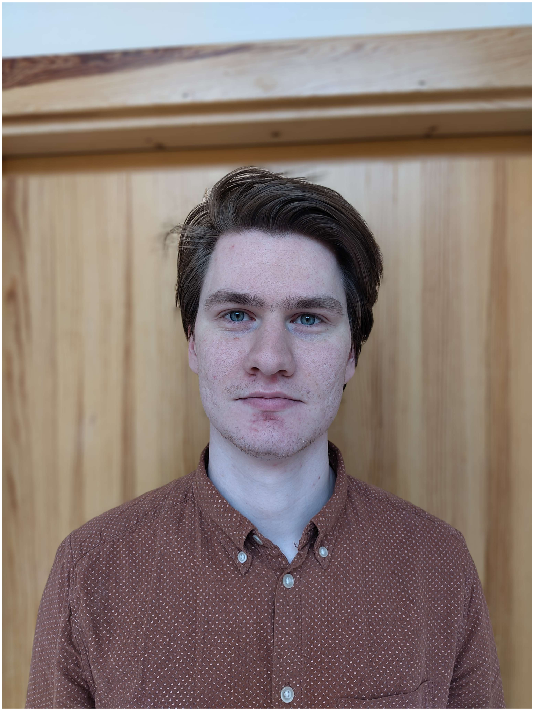
\includegraphics[width=0.3\textwidth]{./YbCbCr_B.png}
    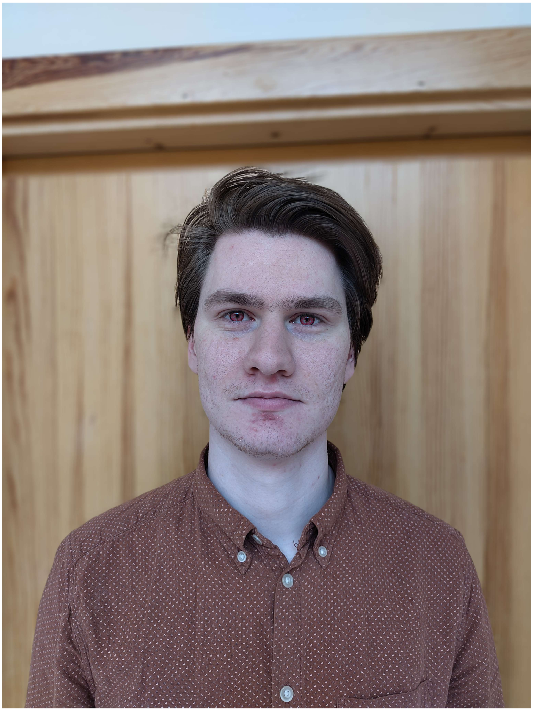
\includegraphics[width=0.3\textwidth]{./YbCbCr_R.png}
    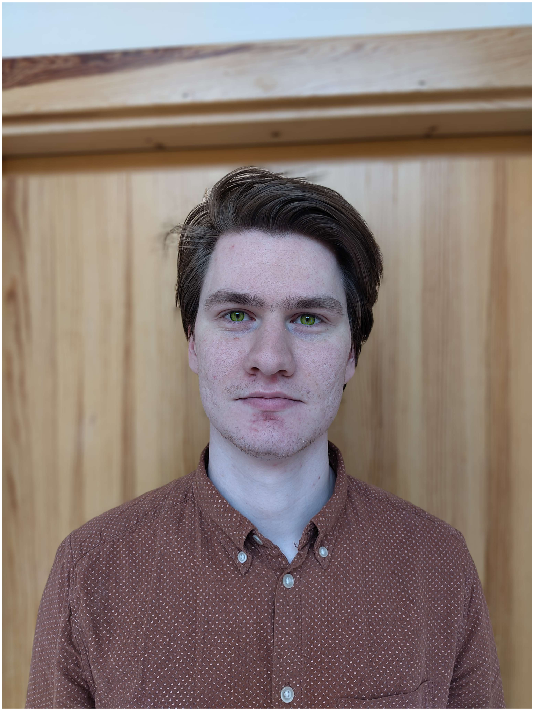
\includegraphics[width=0.3\textwidth]{./YbCbCr_G.png}
    \caption{Left image: The Original image. Middle Image: The red shifted image. Right Image: The green shifted image.}
\end{figure}
\subsection{Conclusion}

The color shifting of the iris is possible but requires mangual cropping, good lighting and certain color spaces to look decent.

\section[Calibration and measurement Calibrate your own camera and undistort ]{Calibration and measurement \\ Calibrate your own camera and undistort}

\subsection{Method}

23 images of a calibration image was taken from varying angles, distances and orientations and inputed into the "Camera Calibration" app. Then the outliers were removed based on the "Mean error pixels" resulting in two images being removed. 

The app then exported a camera parameter file which was used to undistort the images. The efficacy of this undistortion was measured by comparing the length of a pen in the image and compared it to its known length.
\begin{figure}[H]
    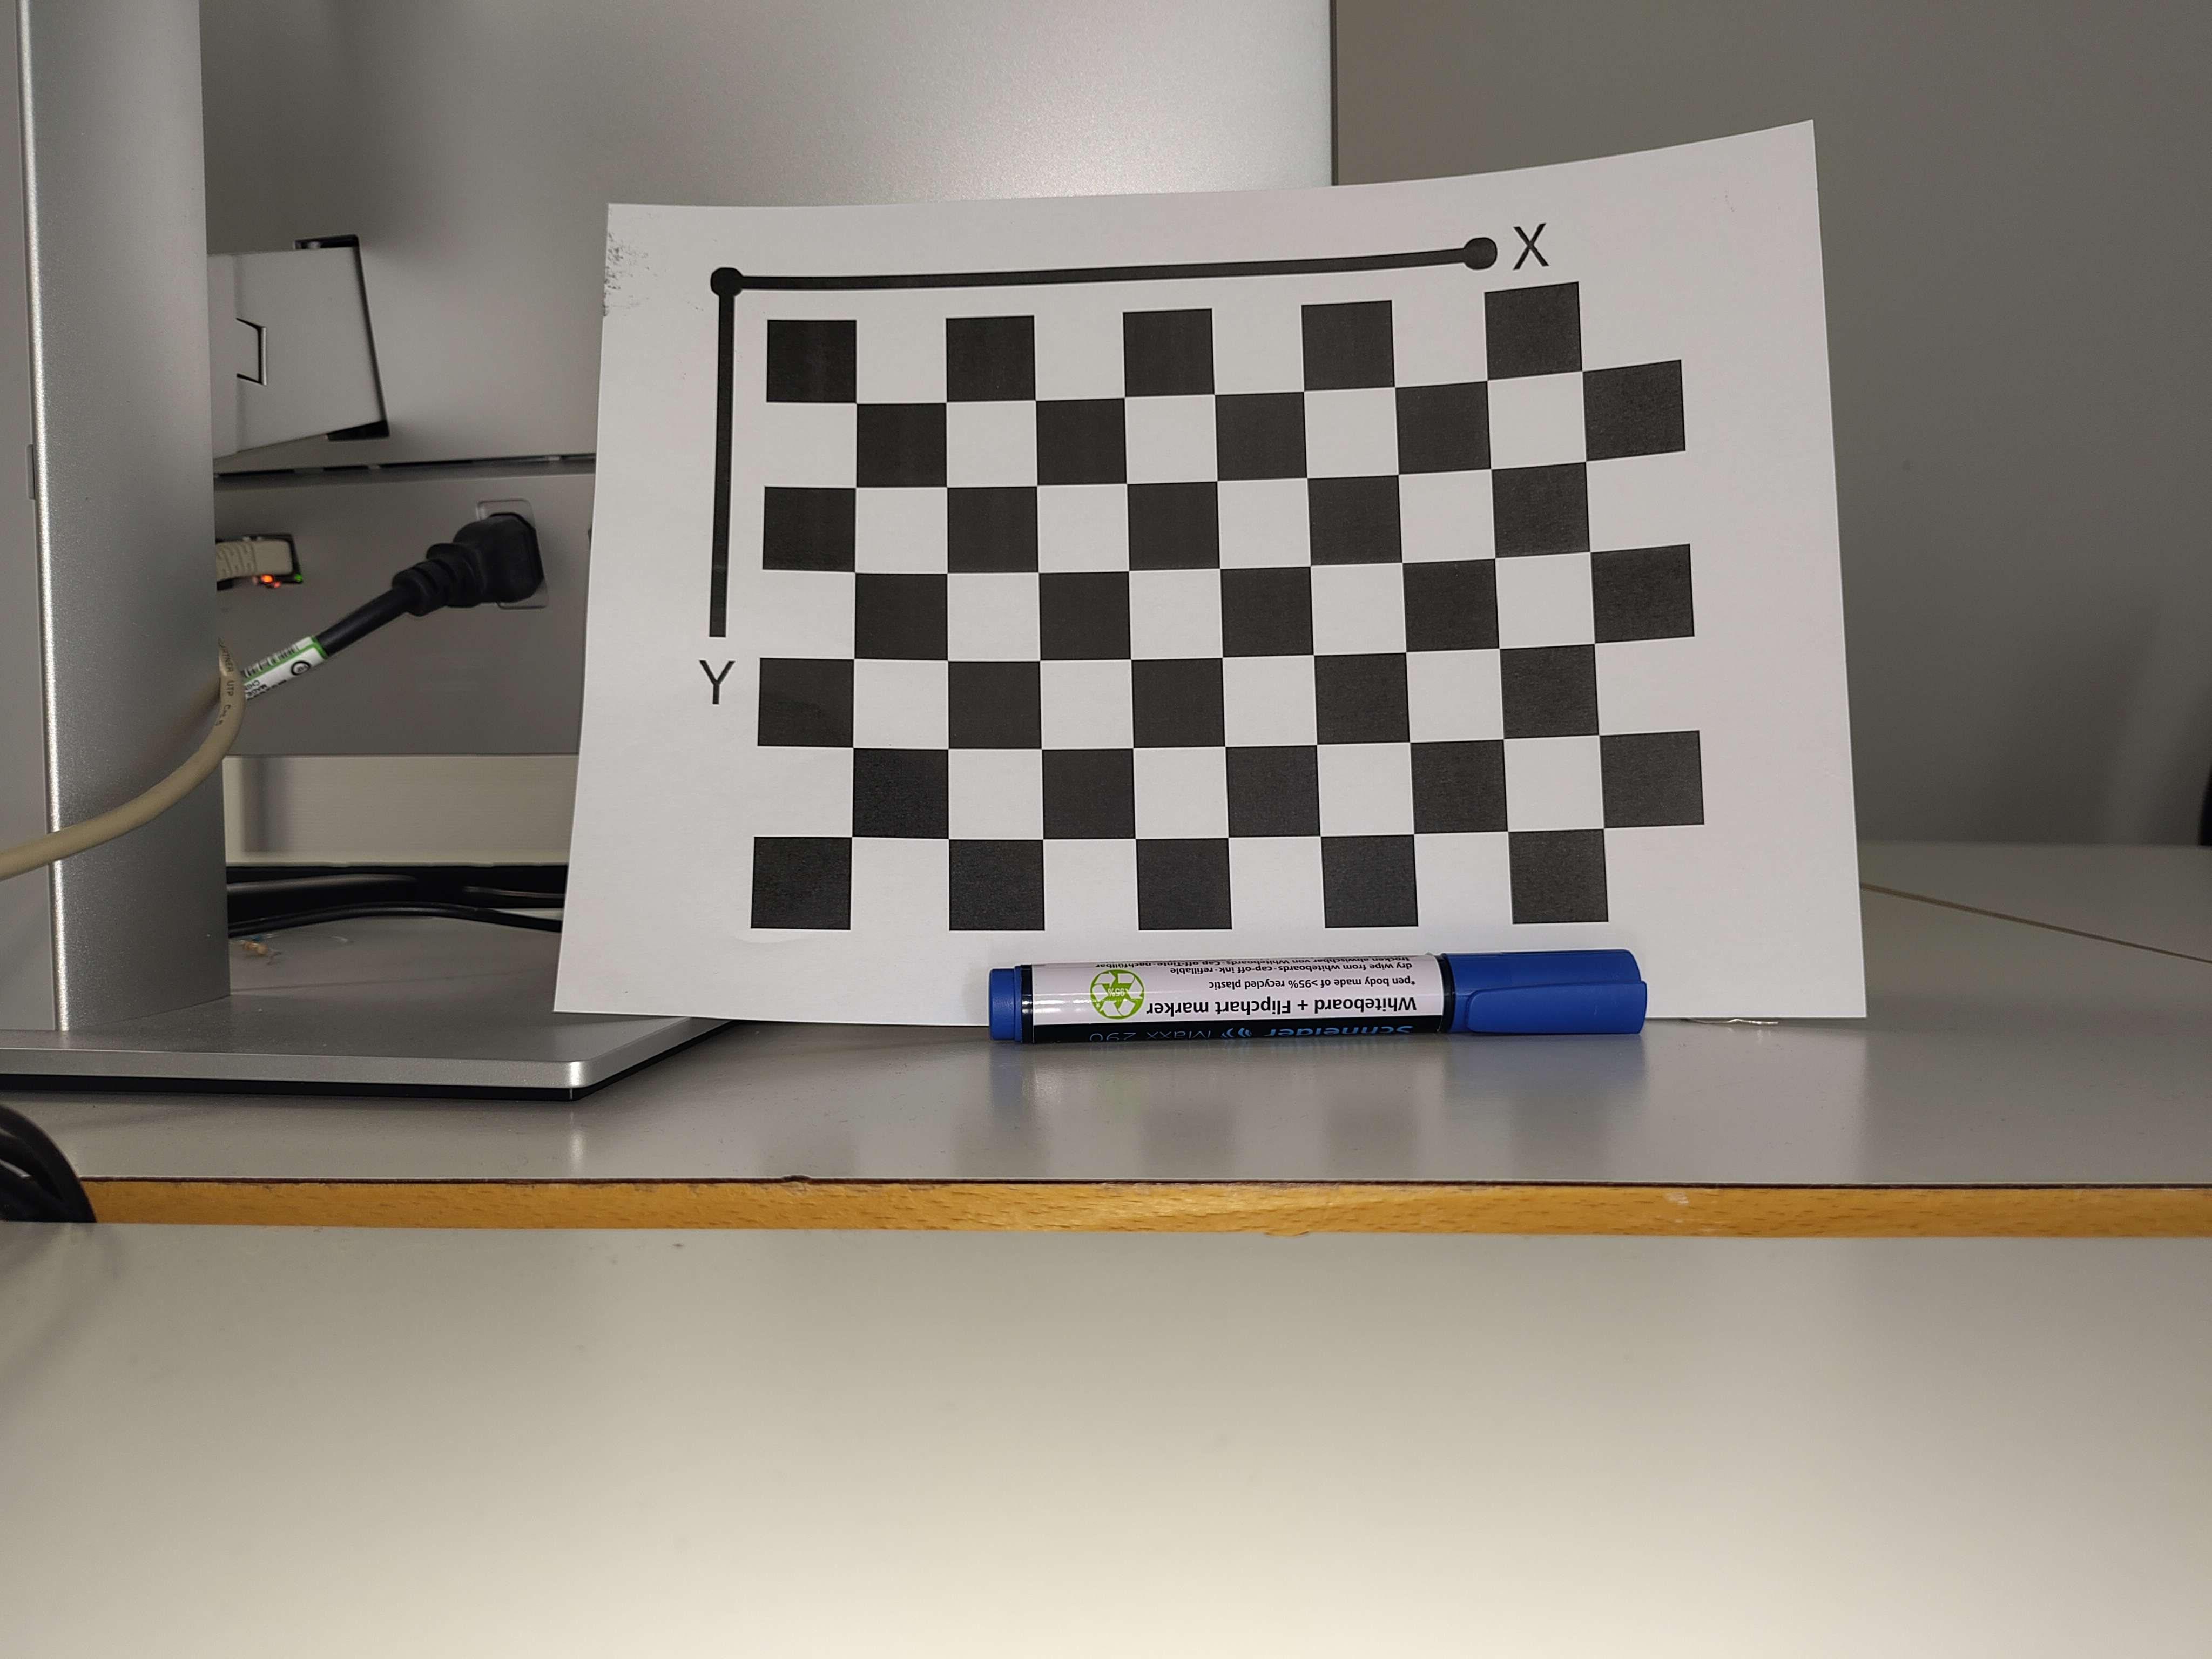
\includegraphics[width=0.4\textwidth]{./Pen1.jpg}
    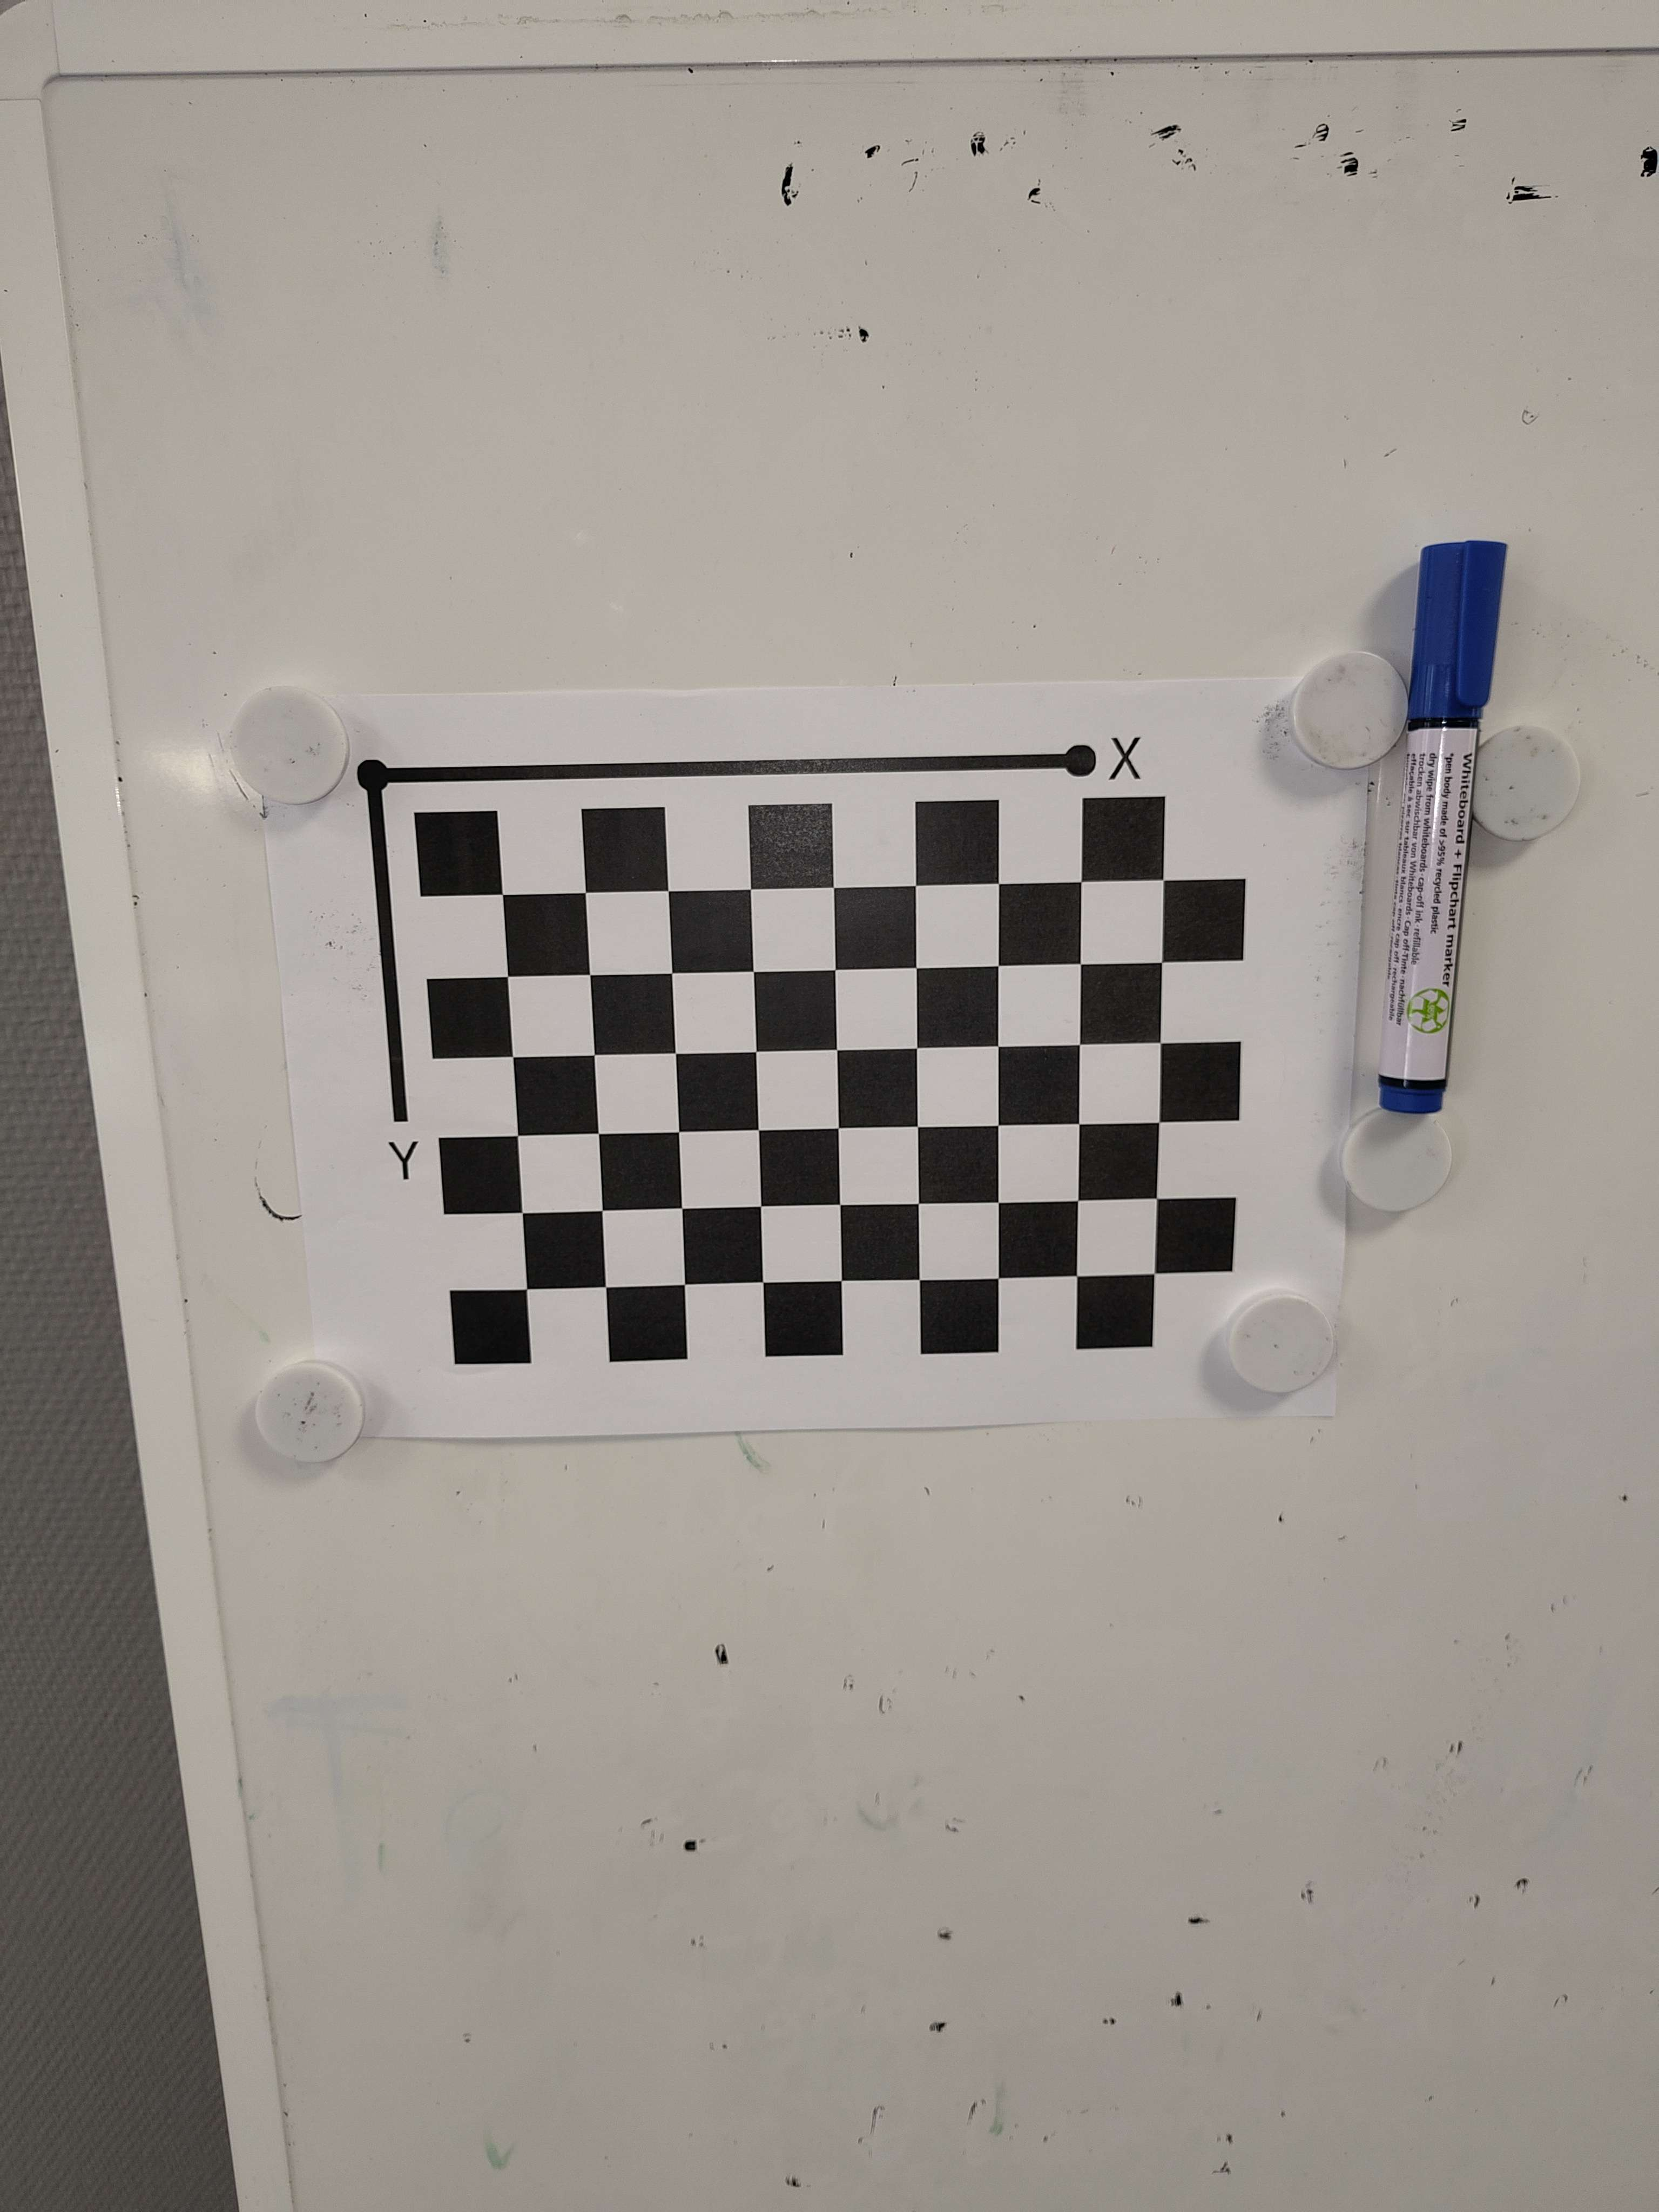
\includegraphics[width=0.4\textwidth]{./Pen2.jpg}
    \caption{The two orignal distorted images}
\end{figure}

The length of the pen and the length of the squares were noted 
\subsection{Result}
The resulting undistorted images:
\begin{figure}[H]
    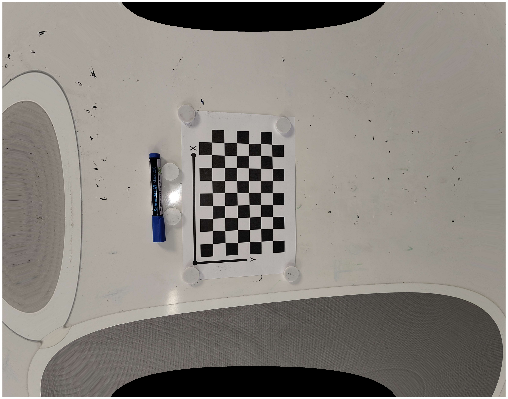
\includegraphics[width=0.4\textwidth, angle = -90]{./Pen1_Undis.png}
    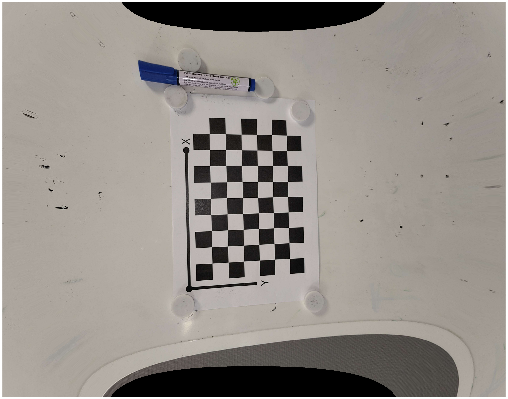
\includegraphics[width=0.4\textwidth, angle = -90]{./Pen2_Undis.png}
    \caption{The two undistorted images}
\end{figure}

\subsection{Conclusion}
